%!TEX root = ../thesis.tex
\chapter{Introduction}
\label{chap:introduction}

The majority of the stars forms in stellar clusters. \citet{2000AJ....120.3139C} reports that $50-70\%$ of very young ($\leq10$ millions of years, in the following Myr) and $25-70\%$ of the young ($\leq100$ Myr) stellar populations are formed in clusters. \citet{2003AJ....126.1916P} and \citet{2003ARA&A..41...57L} find that among 80\% to 90\% of the stars are formed in clusters with more than 100 members. Furthermore, as indicated by the former authors, these clusters ($\geq$100 members) represent 22\% of the regions where stars form. The remaining of the star forming regions are small associations, with 5 to 30 members, where only up to 10\% of the stars are formed. However, only less than 7\% of the clusters ($\geq 100$ members) survives as gravitationally bounded clusters when reaching an age of a few hundred Myr \citep{2003ARA&A..41...57L}. The remaining (93\%) of the star forming regions will become unbounded and their stars will freely populate the galaxy. Thus, to understand the general rules that govern how the majority of stars forms, as well as the properties of the stars that populate our galaxy, it is crucial to fully decode the formation and early evolution of stellar clusters. 

Astrophysicists, like archeologists and palaeontologists, can not willingly reproduce the vast majority of their studied phenomena. Although some experiments can be performed in specific situations (e.g. the chemical and physical  properties of dust and gas) astrophysics remains an observational science. For this reason, to test the validity of their hypotheses, astrophysicists relay on statistical studies carried out over carefully designed observations. In particular, the understanding of the star formation process requires carefully designed observations of  stellar clusters whose ages cover the early stages of cluster evolution.

The objective of this work is the construction, test and validation of an statistical tool, an intelligent system specifically, that given the data of carefully designed observations of an stellar cluster, recovers the statistical distributions of its population. In particular, it delivers the luminosity distribution, which can be transformed into the mass distribution, given an evolutionary model and cluster age. The mass distribution is the fundamental product of the star formation process. It contains the fingerprints of the early phases of star formation and subsequent cluster evolution.

An homogeneous and precise mass distribution inventory for clusters of diverse ages and forming environments will allow the astrophysical community to test the current theories of the star formation process. In particular, it will allow to solve the questions about universality of the initial mass function (IMF, see next Section) and the role play by the physical properties of the cluster environment.    

The remaining of this Chapter is structured as follows. In Section \ref{sect:IMF}, I describe the importance of the initial mass distribution and some of its current models. In Section \ref{sect:numerical_simulations}, I report the current developments of the numerical simulations of cluster formation. In Section \ref{sect:DANCeproject}, I describe the project DANCe and its carefully designed observations of stellar clusters; the ones used in this work. In Section \ref{sect:current_methodologies}, I comment on the current methodologies for the analysis of star clusters and associations. Finally in Section \ref{sect:newtool}, I briefly describe the methodology adopted for this new statistical tool, and the advantages over the previous works. 

\section{The initial mass function of stellar clusters}
\label{sect:IMF}

In his seminal work \citep{Salpeter1955}, Edwin Salpeter defined the \emph{original mass function}, $\xi(M)$, as

\begin{equation}
\rm{d}N= \xi(M)\rm{d}(\log_{10} M) \frac{\rm{d}t}{T_0},
\end{equation}
where $\rm{d}N$ is the number of stars in the mass range $\rm{d}M$ created in the time interval $\rm{d}t$ per cubic parsec, and $T_0$ is the age of the galaxy. Following \citet{Chabrier2003b},  the mass function (MF) at the observed time $t$, is

\begin{equation}
\xi(\log_{10} M)=\frac{\rm{d}N}{\log_{10} M},
\end{equation}

where $N$ is the stellar number density in pc$^{-3}$ and M is the mass. The Initial Mass Function (IMF) is defined as the MF at the time of stellar formation $t=t_0$. The logarithmic transformation,
\begin{equation}
\xi(M)=\frac{1}{M \ln 10} \xi (\log_{10} M),
\end{equation}
is convenient due to the large range of masses covered by the star formation process.

Notice that neither the IMF nor the MF are probability density functions (PDFs) of the mass (see Section \ref{sect:introprobability} for the definition of a PDF). Nevertheless, they can be transformed into PDFs by a normalisation constant, which can be computed by integrating them as functions of the mass over the mass domain. In this work, I will use the PDF of the mass (PDM), denoted by $\xi_L (M)$, as a proxy for the MF. Thus,

\begin{equation}
\xi_L (\log_{10} M) \propto \xi (\log_{10} M)
\end{equation}

The measuring and understanding of the IMF is a central topic in the study of star formation. It is also essential in other areas of astrophysics, from planetary formation, where it appears that the mass of the host star plays an important role in the formation of the planetary system \cite[see for example][]{2015ApJ...814..130M}, to galactic evolution \citep{1998ASPC..142....1K} and cosmology \cite[see for example][]{2012MNRAS.423.3601N}. 

The theories that predict the origin of the IMF can be categorised into deterministic and stochastic \citep{Offner2014}. The former postulate that stellar masses are deterministically inherited from the initial core masses via accretion from the gas reservoir of the parent molecular cloud. Thus, the IMF can be directly mapped from the distribution of initial core masses, and the understanding of the former reduces to that of the latter. On the other hand, stochastic models postulate that the stellar masses are independent of the initial core masses. Among these models, there are those proposing that stellar masses are determined by dynamical interactions and competitive accretion. For more details see \citet{Offner2014} and references therein. 

  The observational studies of the IMF are conditioned on the ages of the stellar populations under analysis (their MF at their corresponding ages), and relay deeply on the assumed processes that link the observed present-day MF to the IMF. While the resulting models for the IMF are always analytical functions of the mass, the observed MF are commonly expressed with points, histograms or kernel density estimations\footnote{KDEs are non-parametric ways to estimate a probability density function by means of an independently and identically distributed sample drawn from it.} (KDEs).

The most common IMFs are the log-normal functions of Chabrier \citep{Chabrier2003a,Chabrier2003b,Chabrier2005}, the power-law functions of Salpeter \citep{Salpeter1955}, Miller and Scalo \citep{1979ApJS...41..513M}, and Kroupa \citep{2001MNRAS.322..231K,2002Sci...295...82K,2013pss5.book..115K,Thies2007,2008MNRAS.390.1200T}. Other functional forms include the truncated exponential \citep{2001AGM....18S0551D} and the Pareto-Levy family distribution \citep{2012MNRAS.423.1018C}. In behalf of simplicity, I will only explain the classical ones of Salpeter, Chabrier, and Kroupa.

\citet{Salpeter1955} derived his famous IMF using a luminosity function resulting from the compilation of the works of \citet{1939POMin...7....1L,1941NYASA..42..201L} and \citet{1925PGro...38D...1V,1936PGro...47....1V}. Then, he transformed it into a MF using a mass-luminosity relation that he obtained after adopting a series of masses and luminosities from the literature. His MF has the form

\begin{equation}
\xi(M)=0.03 \left(\frac{M}{M_{\odot}}\right)^{-1.35},
\end{equation}
with $M$ in the range $0.3\,M_{\odot}$ to  $17\,M_{\odot}$.

\citet{Chabrier2003a,Chabrier2003b} derived his Present-day MF (PDMF) from the nearby luminosity functions of both the $V$ band \citep{1986AJ.....91..621D} and the $K$ band \citep{1990ApJ...350..334H}. He used the \citet{2000A&A...364..217D} and \citet{1998A&A...337..403B} mass-magnitude relations in $V$ and $K$ bands, respectively, to transform the luminosity functions into masses. Then, he fitted a log-normal form to the single objects with masses below 1 $M_{\odot}$. The PDMF he found is,

\begin{equation}
\xi(\log m)_{m\leq1M_{\odot}}=0.158_{-0.046}^{+0.051} \times \exp{\left\{-\frac{(\log m - \log 0.079_{-0.016}^{+0.021})^2}{2 \times (0.69_{-0.01}^{+0.05})^2}\right\}}\ \ (\log M_{\odot})^{-1}\cdot pc^{-3}.\nonumber
\end{equation}

As shown by \citet{1986FCPh...11....1S}, 1 $M_{\odot}$ is the limit at which the PDMF starts to differ from the IMF. Therefore, \citet{Chabrier2003b} uses his PDMF as the IMF below the 1 $M_{\odot}$ limit. Above it, he adopts the Salpeter IMF,

\begin{equation}
\xi(\log m)_{m>1M_{\odot}}= 4.43\times10^{-2}\cdot m^{-1.3\pm0.3}.\nonumber
\end{equation}

As shown by \citet{1991MNRAS.251..293K}, the discrepancies between the luminosity functions derived from photographic samples and from trigonometric parallaxes of nearby stars can be accounted with unresolved binaries. For this reason, \citet{Chabrier2003a} derived the Present-Day system mass function (PDSMF) for unresolved systems. It takes into account each object as a possible unresolved binary or system. This PDSMF has the form,

\begin{equation}
\xi(\log m)_{m\leq1M_{\odot}}=0.086\times \exp{\left\{-\frac{(\log m - \log 0.22)^2}{2 \times (0.57)^2}\right\}}\ \ (\log M_{\odot})^{-1}\cdot pc^{-3},
\end{equation}
with the same normalisation and coefficients of the IMF above 1 $M_{\odot}$.

Later, \citet{Chabrier2005} included in his analysis the revision that \citet{2002AJ....124.2721R} made to the sample of \citep{1986AJ.....91..621D}, and the extended sample of 8 pc from \citet{2004AJ....128..463R}. His new PDMF is

 \begin{align}
\xi(\log m)_{m\leq1M_{\odot}}=&0.093\times \exp{\left\{-\frac{(\log m - \log 0.2)^2}{2 \times (0.55)^2}\right\}}\ \ (\log M_{\odot})^{-1}\cdot pc^{-3},\\
\xi(\log m)_{m>1M_{\odot}}=& 0.041\times m^{-1.3\pm0.3}.
\end{align}

And his new PDSMF is
 \begin{align}
\xi(\log m)_{m\leq1M_{\odot}}=&0.076\times \exp{\left\{-\frac{(\log m - \log 0.25)^2}{2 \times (0.55)^2}\right\}}\ \ (\log M_{\odot})^{-1}\cdot pc^{-3},\\
\xi(\log m)_{m>1M_{\odot}}=& 0.041\times m^{-1.3\pm0.3}.
\end{align}

The canonical IMF of Kroupa \citep{2013pss5.book..115K} is a three-segment power-law, with two segments describing the IMF of the stars, while the third does it for brown-dwarfs (BD). It has the following analytical representation

\begin{align}
\xi_{BD}(m)=&\frac{k}{3}\cdot\left(\frac{m}{0.07}\right)^{-0.3\pm0.4}, \hspace{3.5cm} 0.01M_{\odot} < m \leq 0.15 M_{\odot},\\
\xi(m)=& k\cdot \left(\frac{m}{0.07}\right)^{-1.3\pm0.3}, \hspace{3.5cm} 0.07M_{\odot} < m \leq 0.5 M_{\odot},\\
\xi(m)=& k\cdot \left(\frac{0.5}{0.07}\right)^{-1.3\pm0.3}\cdot  \left(\frac{m}{0.5}\right)^{-2.3\pm0.36}, \ \ \ \ 0.5 M_{\odot} < m \leq 150 M_{\odot},
\end{align}
where $k$ is a constant.
 
 \citet{Thies2007} explored the parametric space of the canonical IMF for different fractions of populations (the number of individual stars and BD) in different clusters: The Trapezium, Taurus, IC 348 and the Pleiades. Figure \ref{fig:IMFThies2007} reproduces their Figure 7. In this Figure, all stellar IMFs are the canonical stellar IMF (previous Equation). However, the IMF for BD corresponds to the optimised one with binary corrections \cite[see][for details]{Thies2007}, with the exception of IC 348 and the Pleiades for which the canonical BD IMF was used. The resulting system IMF is also shown (solid curve).
 
 \begin{figure}[htbp]
\begin{center}
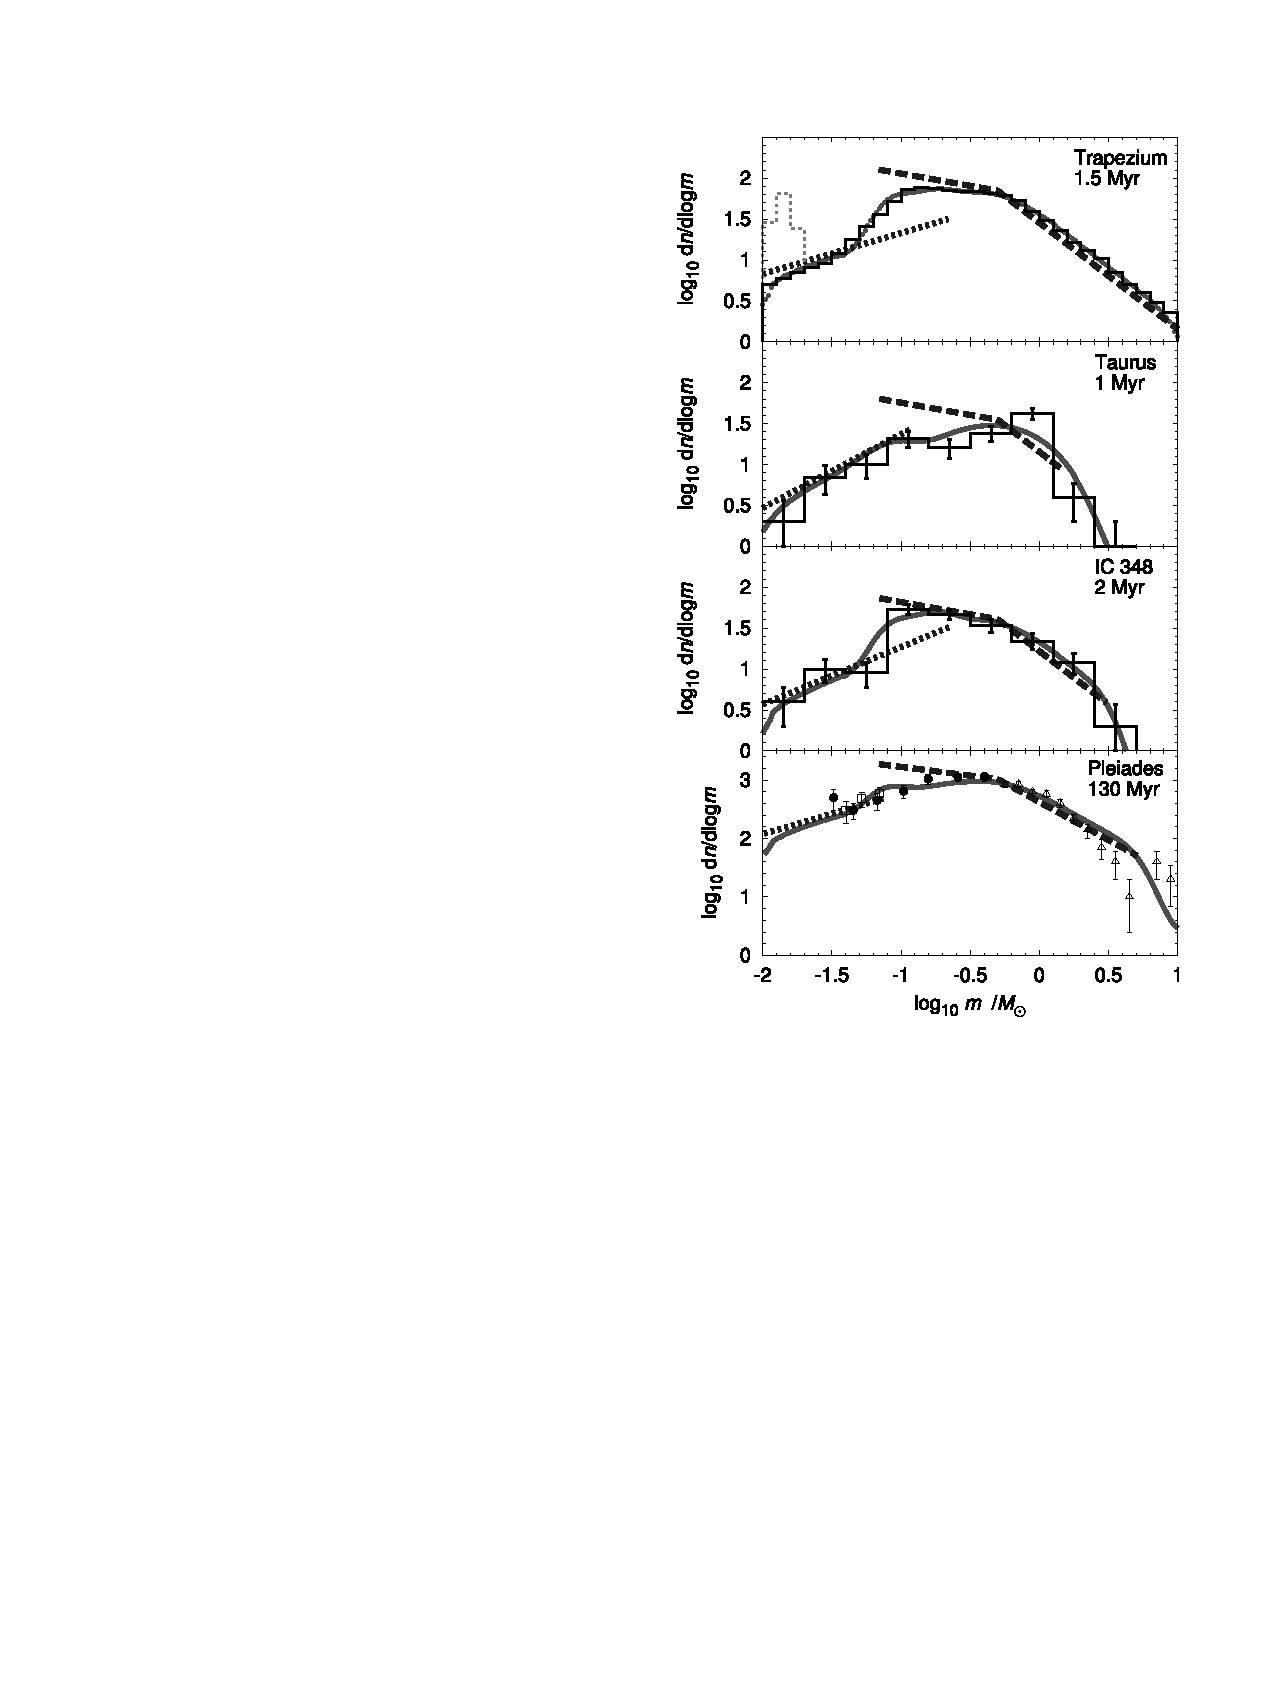
\includegraphics[width=0.8\textwidth]{background/Figures/F7_Thies2007.pdf}
\caption{Observed mass distribution (histograms and dots) together with the stellar (long dashed line), BD (dotted), and system (solid curve) IMFs of \citet{Thies2007} for the Trapezium, Taurus, IC348 and the Pleiades (from top to bottom). Reproduced from Figure 7 of \citet{Thies2007}.}
\label{fig:IMFThies2007}
\end{center}
\end{figure}
 
As shown in this Section, the IMF has been the subject of several studies. However, several questions still remain. In the following section I will explain how the numerical simulations have helped in the understanding of the origin and evolution of the IMF.


\section{Numerical simulations of the early stages of star formation}
\label{sect:numerical_simulations}

In the first decade of this century, numerical simulations of star forming regions have proved to be of paramount importance in the decoding the very early stages of the star formation process \citep{2003MNRAS.339..577B,2005A&A...435..611J,2009MNRAS.392..590B,2009MNRAS.392.1363B,2009MNRAS.397..232B}. For example, \citet{2003MNRAS.339..577B} using smooth particle hydrodynamics were able to simulate the collapse and fragmentation of a large-scale ($50 M_{\odot}$ within 0.375 pc radius) turbulent molecular cloud to from a stellar cluster. During the very first 0.1 Myr of the star formation process, the time covered by the simulation, they were able to simultaneously form discs and binary stars. The cloud formed roughly equal numbers of stars and brown dwarfs (23 and 27, respectively) resulting in a mass distribution with a flat slope in the range $0.01-0.5 M_{\odot}$; see Fig. \ref{fig:IMFBate2003}. \citet{Offner2014} provides a review of the stellar initial mass distribution (function), and of the physical effects included in numerical simulations (radiative feedback, competitive accretion, dynamical interactions, magnetic fields) particularly. 

In recent years, the works of \citet{2015ApJ...815...27K} and \citet{2015MNRAS.452..566B}, using the cold collapse paradigm (neglecting magnetic fields, radiative transfer and feedback), were able to probe that the main source driving the star formation process is gravity. Their simulations were typically run until 0.85 Myr in a box of 3 pc of side, and with masses in the few thousands of $M_{\odot}$. In particular, the mass distribution obtained by \citet{2015ApJ...815...27K} reproduces reasonably well the high mass range of the current models of the initial mass distribution, the IMF of \citet{Chabrier2005} particularly (see Fig. \ref{fig:IMFKuznetsova}). However, compared to this IMF, they produce too few low-mass stars and brown dwarfs.

% Remaining issues

Numerical simulations have proven to be of great use in the understanding of the star formation process in stellar cluster, in the very early phases ( $\leq$1 Myr) of their evolution particularly.  Despite the fact that many of these simulations are in agreement with the observed mass distributions, currently they do not incorporate all astrophysical effects, resolve close binaries or produce enough stellar objects \citep{Offner2014}. 

- The problematic of constraints in dynamical theories.

% Why are these issues important?
\begin{figure}[htbp]
\begin{center}
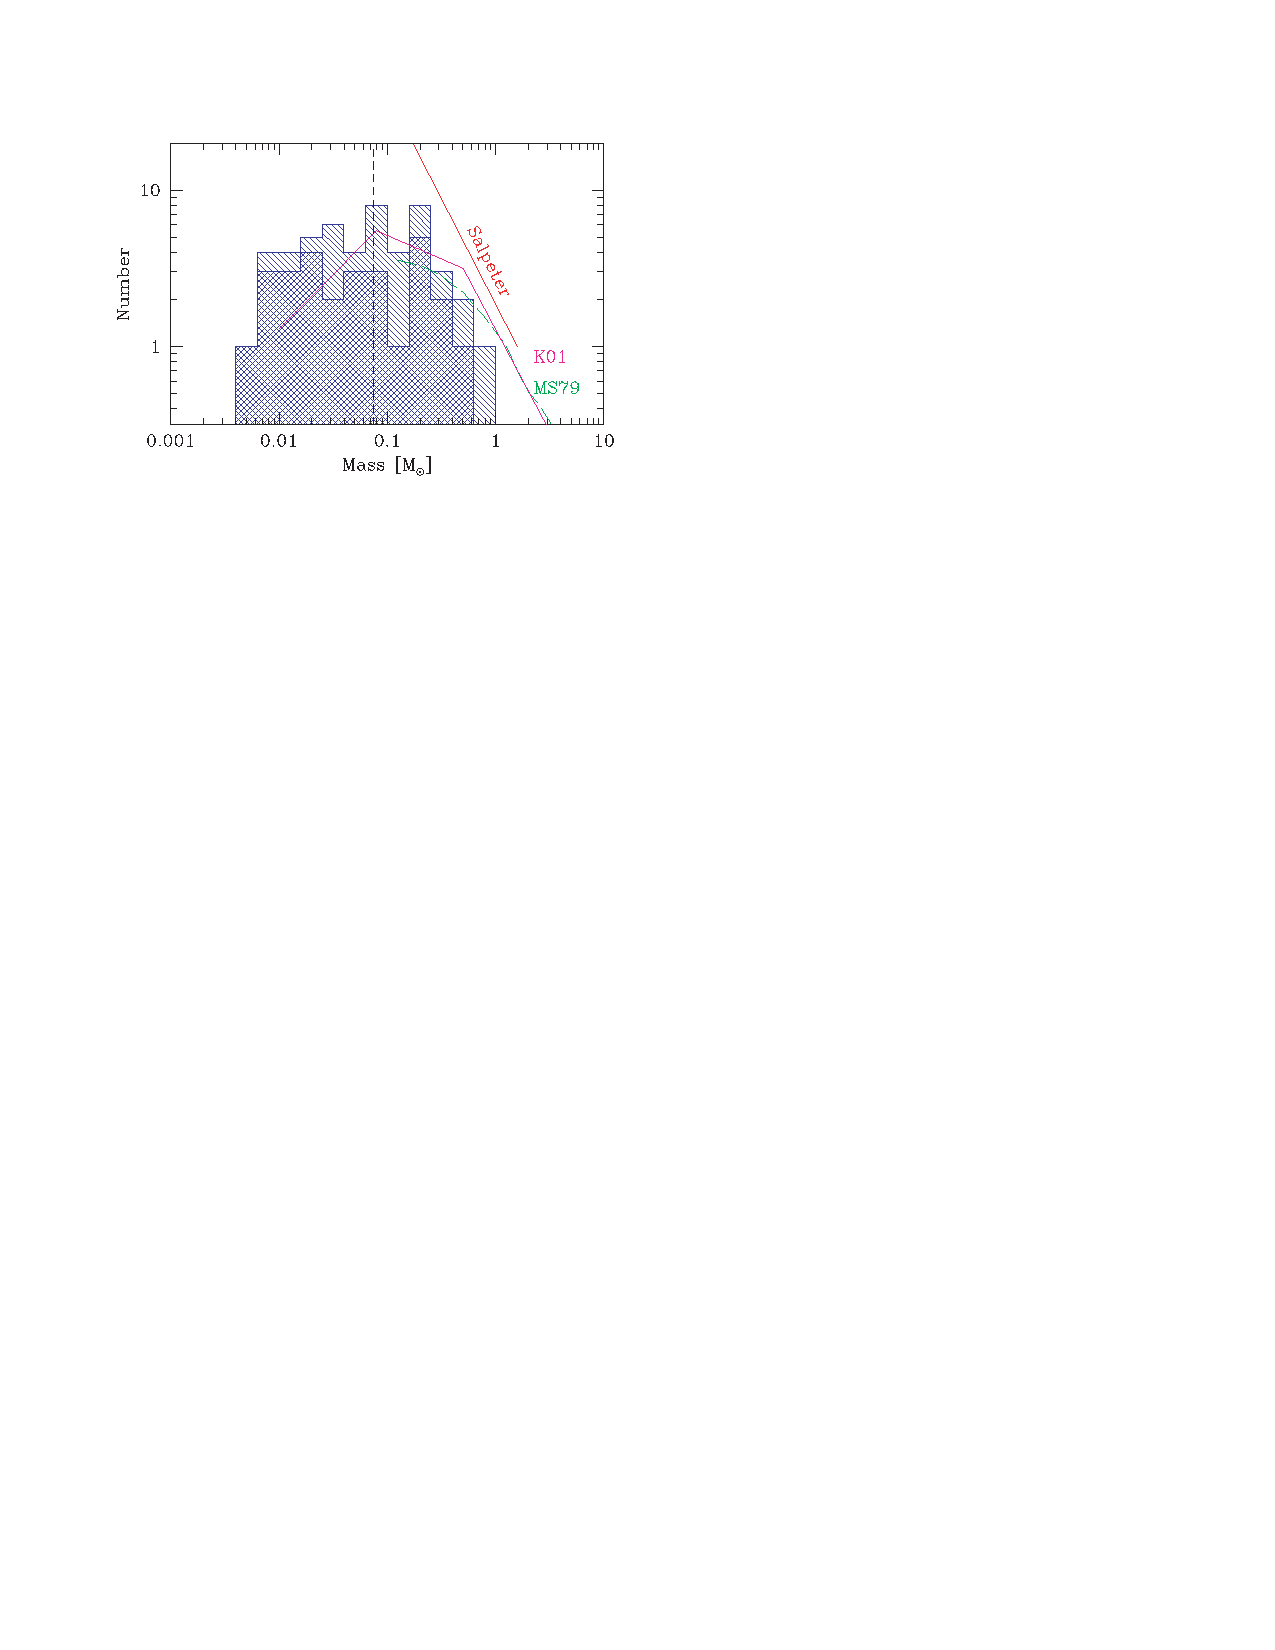
\includegraphics[width=0.8\textwidth]{background/Figures/F10_Bate2003.pdf}
\caption{Mass distribution resulting from the numerical simulation of \citet{2003MNRAS.339..577B}. The lines show the mass distributions of \citet{Salpeter1955}, \citet{1979ApJS...41..513M} and \citet{2001MNRAS.322..231K}. Reproduced from Figure 10 of \citet{2003MNRAS.339..577B}}
\label{fig:IMFBate2003}
\end{center}
\end{figure}

\begin{figure}[htbp]
\begin{center}
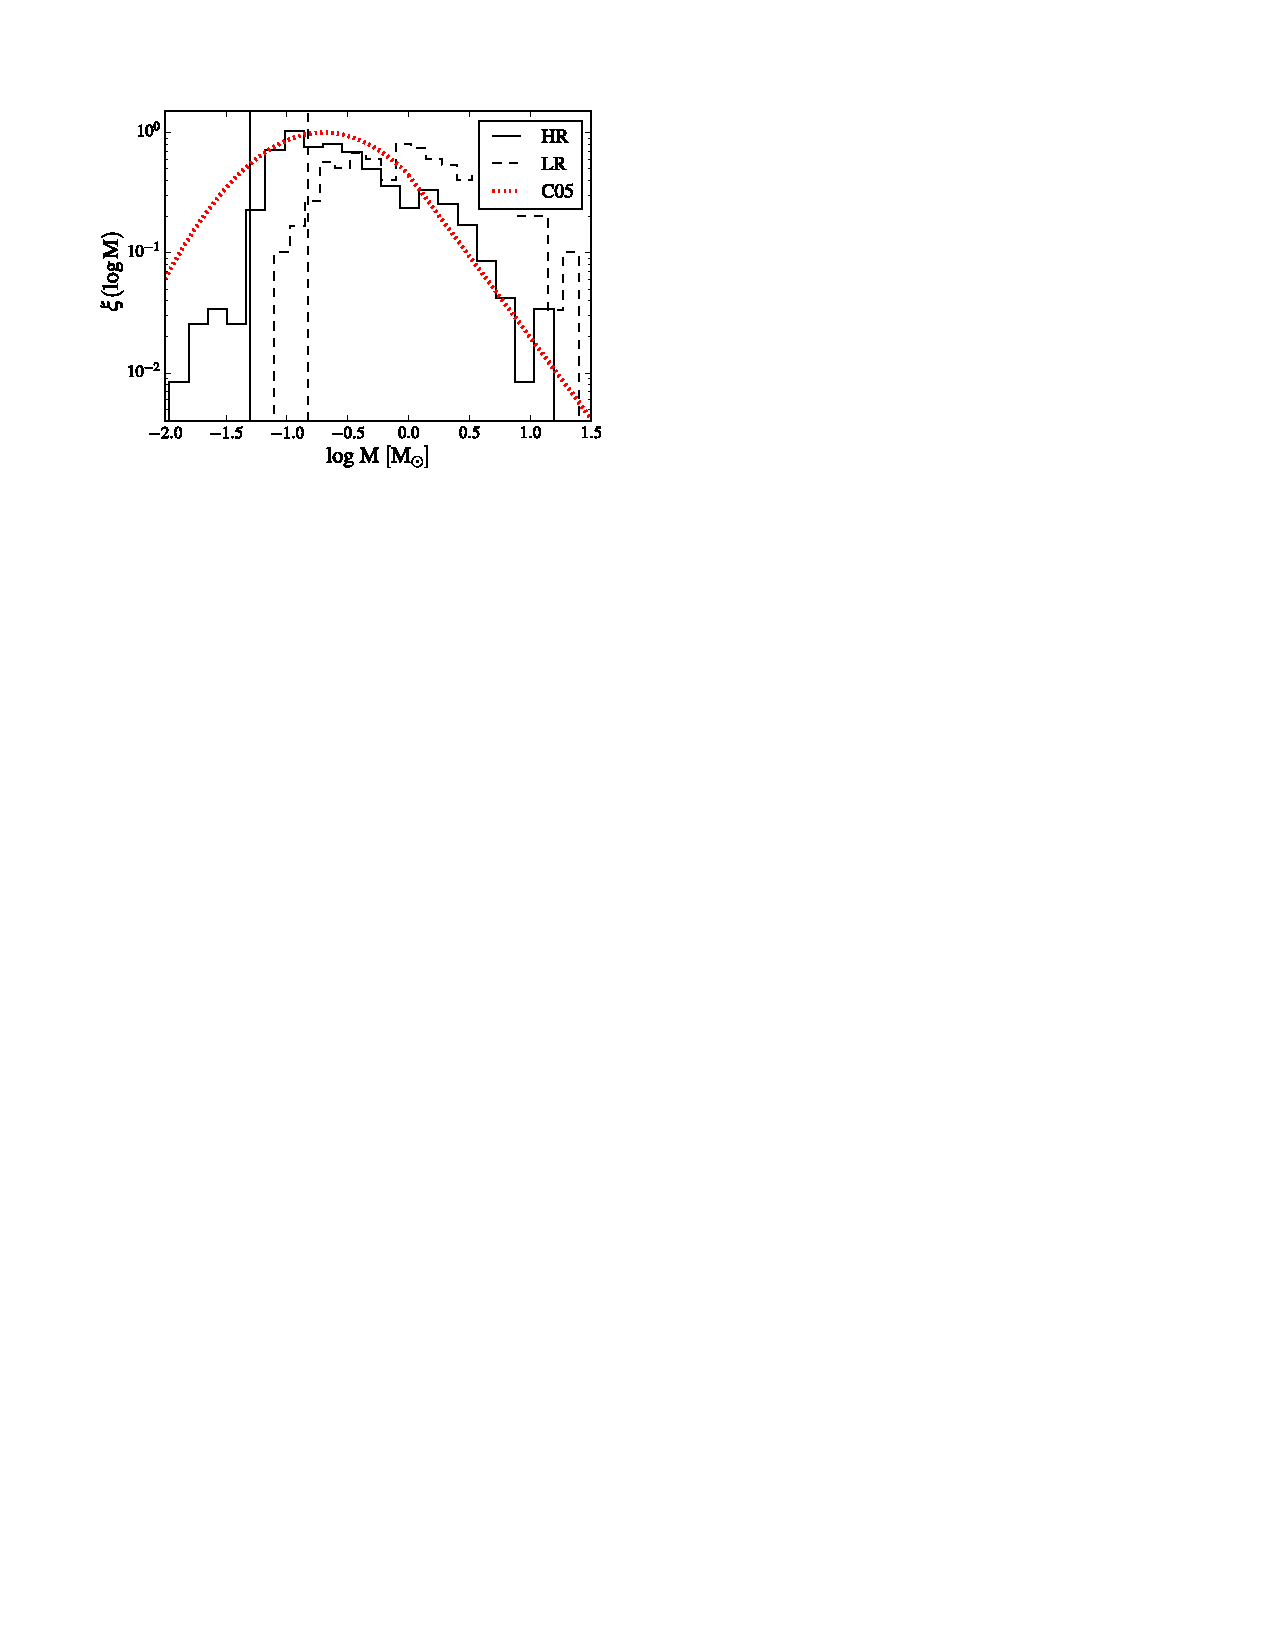
\includegraphics[width=0.8\textwidth]{background/Figures/F11_Kuznetsova2015.pdf}
\caption{Mass distribution resulting from the numerical simulation of \citet{2015ApJ...815...27K}. The High (solid line) and Low (dashed line) resolution simulations reach $0.05\, M_{\odot}$(solid vertical line) and $0.15\, M_{\odot}$ (dashed vertical line), respectively. Also shown the normalised IMF of \citet{Chabrier2005} (red dashed line). Reproduced from Figure 11 of \citet{2015ApJ...815...27K}}
\label{fig:IMFKuznetsova}
\end{center}
\end{figure}

\section{The DANCe project}
\label{sect:DANCeproject}
It must be clear which is the objective

Description of the Nearby open clusters and their properties.

- List of open clusters in the DANce project.

- the importance of the pleiades, why we restrict to it.

It must be clear what are the limitations, the boundaries in which the objective will be searched

\section{Current methodologies}
\label{sect:current_methodologies}
Description of the current methodologies used to address the question mentioned previously.

- The works of Sarro, Krone-Martins, Malo, Gagne etc. LAcweing

-The advantages and caveats of the previous methodologies. 

-It must be clear the necessity of a new perspective

\section{The new tool}
\label{sect:newtool}

The proposal we made. The use of Bayesian Hierarchical Models. Benefits and issues of BHM.

Description of the advantages of BHM.

-> It must be clear that BHM are the best choice.

Description of the practical issues needed to be solved in order to use BHM.

MCMC techniques and  PSO.

-> It must be clear that MCMC methods are the best option.

Brief descriptions of our results and how they impact our current knowledge.

-> It must be clear that we attained the objective: The pleiades velocity, spatial and mass distributions.
 



